\section{Regular expressions for $\TWT$ graphs}\label{sec:reg-exp}


\subsection{Regular expressions for word and multiset graphs}
\begin{definition}[Word and multiset alphabets]
Let $\Sigma_\mathsf{w}$ be the set of terms whose graphs have the following form, where $a,b\in \Sigma_2$ and $c\in \Sigma_1$:
\begin{center}
\includegraphics[scale=.37]{Pictures/word-alphabet}
\end{center}
Let $\Sigma_\mathsf{m}$ be the set of terms whose graphs have the following form, where $a\in \Sigma_2$ and $b\in \Sigma_1$:
\begin{center}
\includegraphics[scale=.35]{Pictures/multiset-alphabet}
\end{center}
 \emph{Word graphs} are the graphs generated from those of $\Sigma_\mathsf{w}$ by series composition,  and \emph{multiset graphs} are the graphs generated from those of $\Sigma_\mathsf{m}$ by parallel composition. 
\end{definition} 
\begin{example}
Below, from left to right, a word graph and two multiset graphs.
\begin{center}
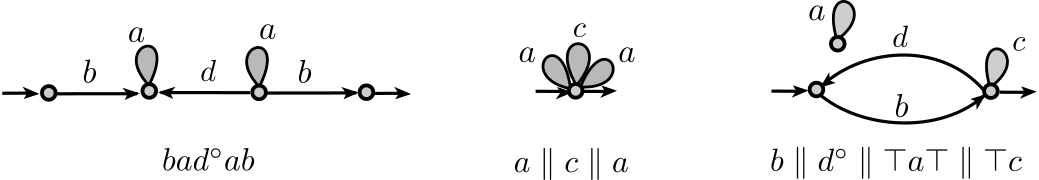
\includegraphics[scale=.4]{Pictures/word-and-multiset-graphs}
\end{center}
\end{example}
\begin{definition}[Word an multiset expressions]
\emph{Word expressions} are defined as follows:
\begin{align*}
\qquad\qquad \qquad e,f := a\ \mid \ e\cdot f\ \mid \ e\cup f\ \mid \ e^+\qquad (a\in \Sigma_\mathsf{w})
\end{align*}
\emph{Multiset pre-expressions} are defined  as follows:
\begin{align*}
\qquad\qquad \qquad e,f := a\ \mid \ (e\parallel f) \ \mid \ e\cup f\ \mid \  e^\parallel\ \qquad (a\in \Sigma_\mathsf{m})
\end{align*}

\emph{Multiset expressions} are those pre-expressions, where each sub-term appearing under a parallel iteration, is built using a  single element $a\in \Sigma_\mathsf{m}$ (all the other operations are allowed). The graph language of an expressions is defined as usual. 
\end{definition}
%We say that a graph language is \emph{word-regular}  or \emph{multiset-regular} if it is the language of a word or a  multiset  regular expression.
\begin{remark}
To see why the condition on multiset regular expressions is useful, consider the expression $e=(a\parll b)$. The language of its parallel iteration is the set of multiset graphs which have the same number of $a$-edges and $b$-edges, and this is  not  a $\CMSO$ definable language. 
\end{remark}


\subsection{Context-free expressions}

\begin{definition}[Context-free expressions]
We define \emph{context-free expressions} as the set of terms generated by the following syntax:
\begin{align*}
\qquad\qquad \qquad e,f := &\ \ \ e_\mathsf{w}\ \mid\ e_\mathsf{m}\\
       & |\ e\cdot f \ \mid\ \  (e \parallel f)\ \ \mid\ \ e^\circ  \ \ \mid\ \dom(e) \ \mid\ 1\ \mid\ \top \\
       & |\ e\cup f \ \mid\  e[f/x] \ \mid\ \mu x. e
\end{align*}
where $e_{\mathsf{w}}$ and $e_{\mathsf{m}}$ are respectively word and multiset regular expressions.  We define the \emph{language} of a context-free expression $e$, denoted $\cL(e)$, by induction on $e$, interpreting the operations of the syntax as described in Sec.~\ref{sec:op-lang}. 
\end{definition}
\emph{Regular expressions for $\TWT$ graphs} will be defined as a restriction of context-free expressions, where substitution and iteration are allowed only under a \emph{guard condition} that we shall explain in the following. 
 



\subsection{The guard condition}

\begin{definition}[Guarded letters]
Let $G$ be a graph and $x$ a letter. We say that:
\begin{itemize}
\item $x$ is \emph{$\mathsf{s}$-guarded in $G$} if $x$ is binary and every $x$-labeled edge of $G$ is parallel to a module.
\item $x$ is \emph{$\mathsf{p}$-guarded in $G$} if $x$ is binary and no $x$-labeled edge of $G$ is parallel to a module.
\item $x$ is $\mathsf{d}$-guarded in $G$ if $x$ is unary.
\item $x$ is $\mathsf{t}$-guarded in $G$ if $x$ is unary and no $x$-labeled edge of $G$ is parallel to a module.
\end{itemize} 
Let $\tau\in\set{\mathsf{s}, \mathsf{p}, \mathsf{d}, \mathsf{t}}$ be a type and $L$ a graph language. We say that \emph{$x$ is $\tau$-guarded} in $L$ if it is $\tau$-guarded in every graph of $L$.
\end{definition}
%\begin{example}
%\todo{add a picture?}
%\end{example}
\begin{definition}[Guard condition] Let $x$ be a letter, $M$ a $\TWT$ graph language and $L$ a pure language of type $\tau$.
The substitution $M[L/x]$ is guarded if $x$ is $\tau$-guarded in $M$.
The iteration $\mu x. L$ is guarded if $x$ is $\tau$-guarded in $L$.

We say that the iteration \emph{$\mu x. L$ is of type $\tau$} if $L$ is of type $\tau$.
\end{definition}


\begin{definition}[Regular expression]
A \emph{regular expression} is a context-free expression where every substitution and iteration is guarded. A language of graphs is \emph{regular} if it is the language of some regular expression. 
\end{definition}
\begin{remark}
When $L$ is test and $x$ is a unary letter, then $\mu x. L$ is always guarded. 
\end{remark}
 

%The following properties show that the guard condition behaves well with substitution and iteration, and that it is a decidable property among context-free expressions.
%
%\begin{proposition}\label{prop:guard-preservation} Let $L$ and $M$  be languages of $\TWT$ graphs. \todo{update}
%\begin{itemize}
%\item If $x$ is guarded in $L$, then $x$ is  guarded in $\mu x. L$.
%\item If $x$ is guarded in $L$ and $M$, then $x$ is guarded in $M[L/x]$.
%\end{itemize}
%\end{proposition}


\begin{proposition}\label{prop:decidability}
We can decide if a  context-free expression is regular.
\end{proposition}
\begin{proof}[Proof sketch]We can annotate our regular expressions with extra information, remembering whether their language is pure, unary, binary, and in
general what type of graphs it generates. This allows us to check the
guard condition and propagate the annotations inductively, using the
syntax tree of the expression.  We start from the leaves of this tree
(labeled by atomic formulas) and propagate the annotations upwards while
verifying the guard condition when required, until we reach the root of
the tree (labeled by the full expression).
\end{proof}
\begin{remark}
Be aware that prop.~\ref{prop:decidability} is about deciding a syntactic property of $e$, namely that the iterations and substitutions are guarded. However, the problem of determining if a context-free expression \emph{defines a $\CMSO$ language} is undecidable. This apparent contradiction comes from the fact that  some context-free expressions, which are not guarded, define $\CMSO$ languages, as we shall see in the upcoming examples.
\end{remark}



\subsection{Examples}



 


\begin{example} The iteration $\mu x. axb$ is not guarded. Indeed, the language of $axb$ is series, as it contains a single series graph $G$. However, the letter $x$ is not $\mathsf{s}$-guarded in $G$, because it is not parallel to any module of $G$. The graph of this iteration look like this:
\begin{center}
\includegraphics[scale=1]{Pictures/expl0.pdf}
\end{center}
\end{example}
 
 \begin{example} The iteration $\mu x. a(x\parallel c)b$ is guarded. Indeed the language of $a(x\parallel c)b$ is series, actually it contains a single graph $G$, depicted below left, which is series. The letter $x$ is $\mathsf{s}$-guarded in $G$, because it is parallel to a module, namely the $c$-edge.   The graph of this iteration look like this:
\begin{center}
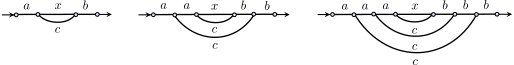
\includegraphics[scale=1]{Pictures/expl1.pdf}
\end{center}
%The language of this expression, while very similar to that of the previous example, is $\CMSO$ definable. 
\end{example}

%It might be surprising that this graph is r somehow the $c$-edges permettent de se repereer dans le graphe. 

Note the similarity between the graph language of $\mu x. axb$ and that of $\mu x. a(x\parallel c)b$: the former is obtained by forgetting the $c$-edges of the latter. Yet, the latter is $\CMSO$ definable, while the former is not. In the case of $\mu x. a(x\parallel c)b$, the $c$-edges will guide a $\CMSO$ formula to relate the $a$-edges and the $b$-edges of the same iteration depth.  This is the main intuition behind the guard condition for series languages.  
%\textcolor{red}{This is a good time to give the intuition on the guard condition.}
 \begin{example}
The iteration $\mu x. (axa\parallel axa)$ is guarded. Indeed, the language of $(axa\parallel axa)$ is parallel, as it contains a unique graph $G$ (the left graph below) which is parallel. The letter $x$ is $\mathsf{p}$-guarded because all the occurrences of $x$ are not parallel to any module of $G$.
Note that the graphs of this expression have the following shape: they all start with  a binary tree whose edges are labeled by $a$, end ends with the mirror image of this tree, while the corresponding leafs are connected by an $x$-edge.  Those trees are colored in red below. 
\begin{center}
\includegraphics[scale=.35]{Pictures/TxT.pdf}
\end{center}
At first glance, this expression dos not seem to be $\CMSO$ definable, as it seems that we need to test whether a graph starts and ends with the same tree. We will see however that the language of this expression, as those of all regular expressions, is $\CMSO$ definable.  
\end{example}

The guard condition is not ``perfect'', in the sense that some non-guarded context-free expressions might  generate $\CMSO$ definable languages, as shown in   the following example.

\begin{example}
 The context-free expression $(\mu x. axb)[1/a, 1/x, 1/b]$ is not regular because the iteration $\mu x. axb$ is not guarded. However its language, the  graph of $1$,   is $\CMSO$ definable.
\end{example}

\begin{remark}
Intuitively, the guard condition allows only those graphs where series and parallel operations alternate. This why we add the word and multiset expressions: to allow graphs where we can iterate only series or parallel operations respectively.
\end{remark}

\subsection{Main result}

The main result of this paper is the following theorem:
\begin{theorem}
Let $L$ be a language of $\TWT$ graphs. We have:
$$L \text{ is recognizable}\qquad \Leftrightarrow \qquad L \text{ is $\CMSO$ definable}  \qquad \Leftrightarrow \qquad L \text{ is regular}$$
%$$\begin{tikzcd}
%               &  L \text{ is recognizable} \arrow[rd, Rightarrow, "(2)"] &  \\[-.5cm]
%L \text{ is $\CMSO$ definable}\arrow[ru, Rightarrow, "(1)"] & \qquad\qquad\qquad\qquad\qquad\qquad\qquad\qquad & L \text{ is regular} \arrow[ll, Rightarrow, "(3)"] 
%\end{tikzcd}$$
%\begin{center}
%$L$ is $\CMSO$-definable $\quad\Leftrightarrow\quad$ $L$ is recognizable $\quad\Leftrightarrow\quad$ $L$ is regular
%\end{center}
\end{theorem}
Thanks to Thm.~\ref{thm:CMSO->Rec}, $\CMSO$ definability implies recognizablity. We show that regularity implies $\CMSO$ definability in Sec.~\ref{sec:reg->def} and  that recognizabilty implies regularity in Sec.~\ref{sec:rec->reg}. 